\documentclass{beamer}
\usepackage{graphicx}
\usepackage{xcolor}
\usepackage{amsmath}
\usepackage{ctex}
\usepackage{amssymb}
\usepackage{xeCJK}

\title{Operating System Seminar}
\subtitle{Bootloader}
\institute{University of Chinese Academy of Sciences}
\author{冯吕,张旭}
\date{\today}
\usetheme{PaloAlto}
\begin{document}
\zihao{5}
\CJKfamily{zhkai}
\begin{frame}
\titlepage
\begin{figure}[ht]\centering
\includegraphics[scale=0.3]{ucas.jpg}\end{figure}
\end{frame}

\begin{frame}{Outline}
\tableofcontents
\end{frame}
 
\section{task2}
\begin{frame}{Task2 任务}
通过向串口输出字符串实现开发板$BIOS$调用。

\end{frame}

\begin{frame}{实现方法}
不断向串口输出地址 $0xbfe48000$处写字符。
\end{frame}

\begin{frame}{代码实现}
开始时在 $.data$段定义了一个字符串变量:\\ \textbf{str: .asciiz "Welcome to OS!"}

\begin{figure}

	\centering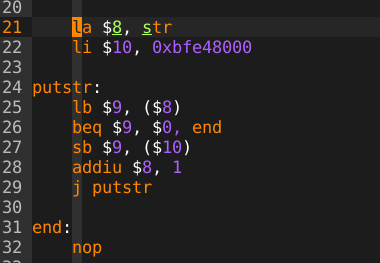
\includegraphics[scale=0.6]{putstr.png}
\end{figure}
\end{frame}

\section{task3}
\begin{frame}{task3 任务}
实现一个操作系统启动程序。	

启动程序被放在了启动设备的第一个扇
区,系统启动时该扇区被 $loadboot $自动加载在内存地址 $0xa0800000 $处,然后
从它的入口地址$ 0xa0800030 $开始执行。启动程序需要将剩余的操作系统程序加
载的内存中,即内核。	
\end{frame}

\begin{frame}{实现}
\begin{enumerate}
	\item 向读盘函数传递参数。
	\begin{itemize}
		\item 参数$1$:内存存放地址$(0xa0800200)$
		\item 参数$2$:$SD$卡偏移量$(512)$
		\item 参数$3$:需要读取的字节数$(512)$
	\end{itemize}
	\item 调用读盘函数。
	\item 跳到内核的开始处执行(实际是调用内核的$main$函数)
\end{enumerate}
\end{frame}

\begin{frame}{代码实现}
\begin{figure}
	
	\centering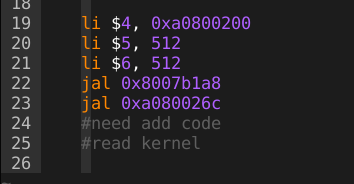
\includegraphics[scale=0.6]{load.png}
\end{figure}
\end{frame}

\begin{frame}{错误分析}
刚开始的时候跳到内核开始处执行使用了$J$指令,导致不停输出\emph{It's kernel}。

原因(个人理解):在上一次调用读盘函数的时候,返回地址保存到了$31$号寄存器,之后使用$J$指令跳转
到内核处执行的时候不是函数调用,因此$31$号寄存器的值没有更新,所以从内核返回的时候又回到了之前的地方,
导致不断循环调用内核中的$main$函数。
\end{frame}

\section{task4}
\begin{frame}{任务}
实现一个 $Linux$工具,将启动程序和内核编译为一个$ MIPS$ 架构支持的操作
系统镜像。
	
\end{frame}

\begin{frame}{代码实现}{read\_exec\_file 函数}
\begin{figure}
	
	\centering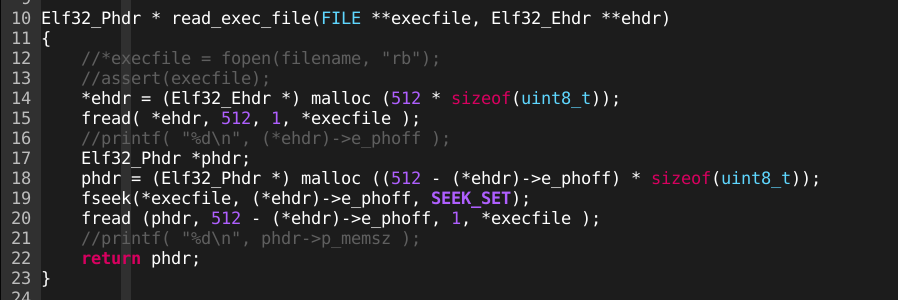
\includegraphics[scale=0.3]{read.png}
\end{figure}
调用函数:$malloc, fread, fseek$.

首先分配一个缓冲区,读取$512$个字节进去,然后便可知道文件头表。之后重新分配一个缓冲区,将文
件指针移动到程序段的开始处,读取内容,然后便获得了程序头表。
\end{frame}

\begin{frame}{代码实现}{count\_kernel\_sectors}
\begin{figure}
	
	\centering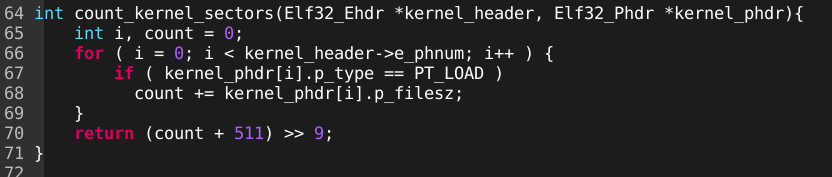
\includegraphics[scale=0.3]{count.png}
\end{figure}
直接看代码!

\end{frame}

\begin{frame}{代码实现}

\begin{figure}
	
	\centering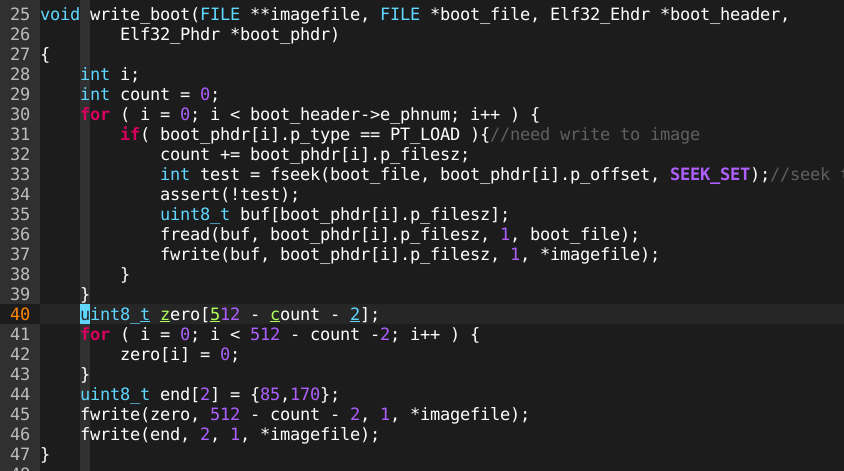
\includegraphics[scale=0.3]{wboot.png}
\end{figure}
$write\_boot$和$write\_kernel$:二者区别不大。不同的地方是在第一个扇区的结束的最后两个
字节应写上$0x55$和$0xaa$。

看代码。
\end{frame}

\begin{frame}{$main$函数}
\begin{figure}
	
	\centering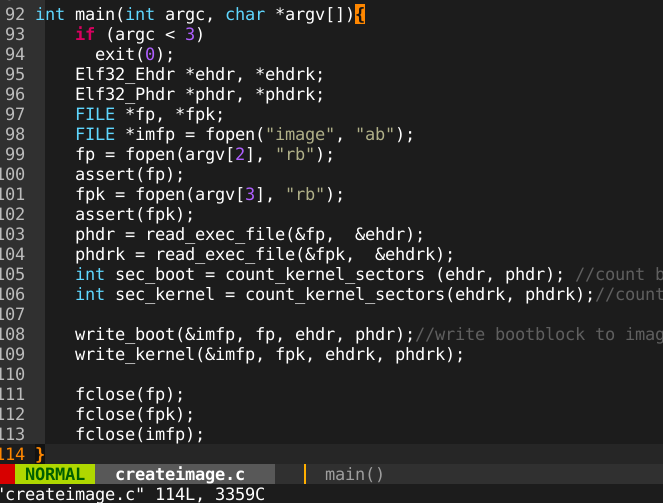
\includegraphics[scale=0.3]{mainm.png}
\end{figure}
首先调用$read\_exec\_file$函数读取可执行文件,然后将相应的内容写入镜像文件中。
\end{frame}

\begin{frame}{extended\_opt函数}
根据之前的读取信息和计算扇区数的函数即可打印出相关的信息。
\begin{figure}
	
	\centering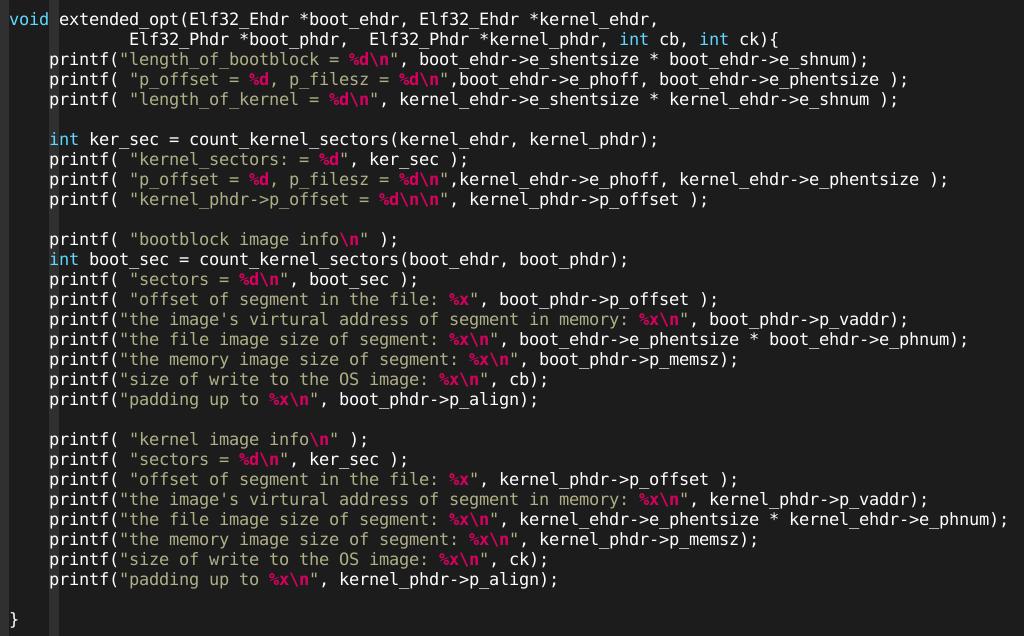
\includegraphics[scale=0.25]{et.png}
\end{figure}
\end{frame}

\begin{frame}{未实现函数}
$record\_kernel\_sectors$函数还未实现。

如何向$bootblock$传参?嵌入式汇编?


\end{frame}

\end{document}